%&tex

\documentclass{beamer}

\usepackage[english]{babel}
\usepackage[utf8]{inputenc}
\usepackage{mathtools}
\usepackage{amsthm}
\usepackage{amssymb}
\usepackage{thmtools,thm-restate}
\usepackage{amsfonts}
\usepackage{hyperref}
\usepackage[singlelinecheck=false]{caption}
\usepackage[backend=biber,url=true,doi=true,eprint=false,style=authoryear]{biblatex}
\usepackage{algorithm}
\usepackage[noend]{algpseudocode}
\usepackage{listings}
\usepackage{subcaption}
\usepackage{xcolor}

\usepackage{graphicx}
\usepackage{tikz}
\usetikzlibrary{positioning}
\usetikzlibrary{shapes.geometric}
\usetikzlibrary{fit}
\usetikzlibrary{calc}

\usepackage{tkz-graph}

\addbibresource{references.bib}
\usetheme{metropolis}

\DeclareMathOperator*{\argmin}{arg\,min}
\DeclareMathOperator*{\argmax}{arg\,max}
\DeclareMathOperator*{\Val}{\text{Val}}
\DeclareMathOperator*{\Ch}{\text{Ch}}
\DeclareMathOperator*{\Pa}{\text{Pa}}
\DeclareMathOperator*{\Sc}{\text{Sc}}
\newcommand{\ov}{\overline}
\newcommand{\tsup}{\textsuperscript}

\newcommand\defeq{\mathrel{\overset{\makebox[0pt]{\mbox{\normalfont\tiny\sffamily def}}}{=}}}

\newcommand{\algorithmautorefname}{Algorithm}
\algrenewcommand\algorithmicrequire{\textbf{Input}}
\algrenewcommand\algorithmicensure{\textbf{Output}}
\algnewcommand{\LineComment}[1]{\State\,\(\triangleright\) #1}

\newcommand{\Left}{\text{LEFT}}
\newcommand{\Right}{\text{RIGHT}}
\newcommand{\Up}{\text{UP}}

\newcommand{\set}[1]{\mathbf{#1}}
\newcommand{\pr}{\text{P}}
\newcommand{\eps}{\varepsilon}
\newcommand{\ddspn}[2]{\frac{\partial#1}{\partial#2}}
\newcommand{\iddspn}[2]{\partial#1/\partial#2}
\newcommand{\indep}{\perp}
\renewcommand{\implies}{\Rightarrow}

\newcommand{\bigo}{\mathcal{O}}
\newcommand{\mbf}[1]{\mathbf{#1}}

\setbeamertemplate{theorems}[ams style]

\setbeamersize{description width=1.0cm}

\lstset{frameround=fttt,
	numbers=left,
	breaklines=true,
	keywordstyle=\bfseries,
	basicstyle=\ttfamily,
}

\newcommand{\code}[1]{\lstinline[mathescape=true]{#1}}
\newcommand{\mcode}[1]{\lstinline[mathescape]!#1!}

\title{Mobile Robot Self-Driving Through Image Classification Using Sum-Product Networks}
\date{}
\author{Student: Renato Lui Geh\\Advisor: Prof. Dr. Denis Deratani Mauá}
\institute{Institute of Mathematics and Statistics --- University of São Paulo}

\begin{document}

\maketitle

\section{Sum-Product Networks}

\begin{frame}
  \frametitle{Definition}
  \begin{definition}[Sum-product network]~\\
    A sum-product network (SPN) is a DAG where each node $n$ is either:
    \begin{enumerate}
      \item A tractable univariate probability distribution;
      \item A product of SPNs: $v_n=\prod_{j\in\Ch(n)}v_j$; or
      \item A weighted sum of SPNs: $v_n=\sum_{j\in\Ch(n)}w_{n,j}v_j$.
    \end{enumerate}
    Where $v_n$ is the value of node $n$, $\Ch(n)$ its set of children and $w_{n,j}$ the weight of
    edge $n\to j$.
  \end{definition}
\end{frame}

\begin{frame}
  \frametitle{Example}

  \textbf{Sums} can be interpreted as \emph{mixture models} and \textbf{products} as their
  \emph{components}.  \textbf{Leaves} can take the form of categorical or continuous
  \emph{distributions}.

  \begin{center}
    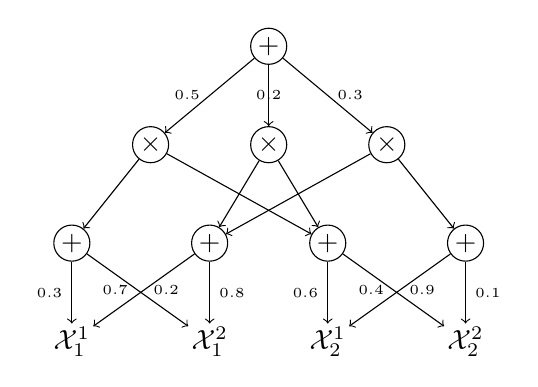
\begin{tikzpicture}
      \begin{scope}[every node/.style={circle,draw,inner sep=1pt}]
        \node (root) at (0, 0) {+};
        \node (p1) at (-1.5, -1.25) {$\times$};
        \node (p2) at (0, -1.25) {$\times$};
        \node (p3) at (1.5, -1.25) {$\times$};
        \node (s1) at (-2.5, -2.5) {+};
        \node (s2) at (-0.75, -2.5) {+};
        \node (s3) at (0.75, -2.5) {+};
        \node (s4) at (2.5, -2.5) {+};
        \node[draw=none,fill=none,rectangle] (x11) at (-2.5, -3.75) {$\mathcal{X}_1^1$};
        \node[draw=none,fill=none,rectangle] (x12) at (-0.75, -3.75) {$\mathcal{X}_1^2$};
        \node[draw=none,fill=none,rectangle] (x21) at (0.75, -3.75) {$\mathcal{X}_2^1$};
        \node[draw=none,fill=none,rectangle] (x22) at (2.5, -3.75) {$\mathcal{X}_2^2$};
      \end{scope}

      \begin{scope}[every path/.style={->}]
        \draw (root) -- node[left]{\tiny$0.5$} (p1);
        \draw (root) -- node{\tiny$0.2$} (p2);
        \draw (root) -- node[right]{\tiny$0.3$} (p3);
        \draw (p1) -- (s1);
        \draw (p1) -- (s3);
        \draw (p2) -- (s2);
        \draw (p2) -- (s3);
        \draw (p3) -- (s2);
        \draw (p3) -- (s4);
        \draw (s1) -- node[left]{\tiny$0.3$} (x11);
        \draw (s1) -- node[left]{\tiny$0.7$} (x12);
        \draw (s2) -- node[right]{\tiny$0.2$} (x11);
        \draw (s2) -- node[right]{\tiny$0.8$} (x12);
        \draw (s3) -- node[left]{\tiny$0.6$} (x21);
        \draw (s3) -- node[left]{\tiny$0.4$} (x22);
        \draw (s4) -- node[right]{\tiny$0.9$} (x21);
        \draw (s4) -- node[right]{\tiny$0.1$} (x22);
      \end{scope}
    \end{tikzpicture}
  \end{center}

  Where each leaf $\mathcal{X}_i^j$ is a probability distribution over RV $X_i$.

\end{frame}

\begin{frame}
  \frametitle{Scope}

  The scope $\Sc(n)$ of node $n$ is the union of the scope of its children. The scope of a leaf is
  the set of all variables in the distribution. Let $S$ be the root of the SPN below:
  \vspace{-0.75cm}

  \begin{center}
    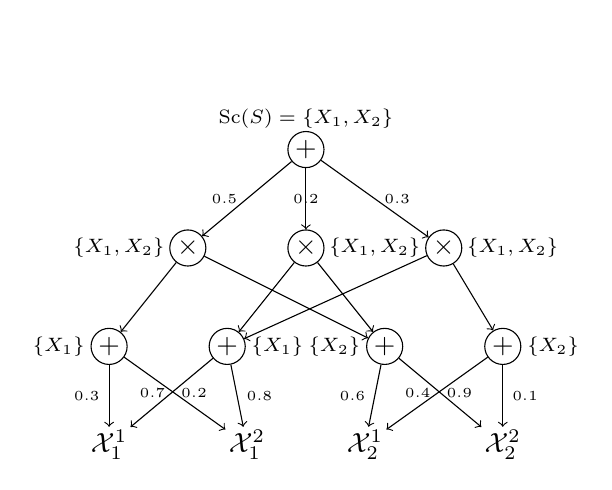
\begin{tikzpicture}
      \begin{scope}[every node/.style={circle,draw,inner sep=1pt}]
        \node[label={[label distance=-1.0cm]above:{\scriptsize$\Sc(S)=\{X_1,X_2\}$}}] (root) at (0, 0) {+};
        \node[label=left:{\scriptsize$\{X_1,X_2\}$}] (p1) at (-1.5, -1.25) {$\times$};
        \node[label=right:{\scriptsize$\{X_1,X_2\}$}] (p2) at (0, -1.25) {$\times$};
        \node[label=right:{\scriptsize$\{X_1,X_2\}$}] (p3) at (1.75, -1.25) {$\times$};
        \node[label=left:\scriptsize$\{X_1\}$] (s1) at (-2.5, -2.5) {+};
        \node[label=right:\scriptsize$\{X_1\}$] (s2) at (-1.0, -2.5) {+};
        \node[label=left:\scriptsize$\{X_2\}$] (s3) at (1.0, -2.5) {+};
        \node[label=right:\scriptsize$\{X_2\}$] (s4) at (2.5, -2.5) {+};
        \node[draw=none,fill=none,rectangle] (x11) at (-2.5, -3.75) {$\mathcal{X}_1^1$};
        \node[draw=none,fill=none,rectangle] (x12) at (-0.75, -3.75) {$\mathcal{X}_1^2$};
        \node[draw=none,fill=none,rectangle] (x21) at (0.75, -3.75) {$\mathcal{X}_2^1$};
        \node[draw=none,fill=none,rectangle] (x22) at (2.5, -3.75) {$\mathcal{X}_2^2$};
      \end{scope}

      \begin{scope}[every path/.style={->}]
        \draw (root) -- node[left]{\tiny$0.5$} (p1);
        \draw (root) -- node{\tiny$0.2$} (p2);
        \draw (root) -- node[right]{\tiny$0.3$} (p3);
        \draw (p1) -- (s1);
        \draw (p1) -- (s3);
        \draw (p2) -- (s2);
        \draw (p2) -- (s3);
        \draw (p3) -- (s2);
        \draw (p3) -- (s4);
        \draw (s1) -- node[left]{\tiny$0.3$} (x11);
        \draw (s1) -- node[left]{\tiny$0.7$} (x12);
        \draw (s2) -- node[right]{\tiny$0.2$} (x11);
        \draw (s2) -- node[right]{\tiny$0.8$} (x12);
        \draw (s3) -- node[left]{\tiny$0.6$} (x21);
        \draw (s3) -- node[left]{\tiny$0.4$} (x22);
        \draw (s4) -- node[right]{\tiny$0.9$} (x21);
        \draw (s4) -- node[right]{\tiny$0.1$} (x22);
      \end{scope}
    \end{tikzpicture}
  \end{center}

\end{frame}

\begin{frame}
  \frametitle{Validity}

  \begin{definition}[Validity]~\\
    Let $S$ be an SPN. If $S$ correctly computes and marginalizes an unnormalized probability
    $\phi(\mbf{X})$, then it is said to be \emph{valid}.
  \end{definition}~\\

  If for every sum node $n$

  \begin{equation*}
    \forall j\in\Ch(n), w_{n,j} \geq 0\text{ and }\sum_{j\in\Ch(n)}w_{n,j} = 1
  \end{equation*}

  then $S$ represents the probability distribution itself.\\~\\

  A sufficient, yet not necessary, condition for validity is \emph{completeness} and
  \emph{consistency} (\cite{poon-domingos}).

\end{frame}

\begin{frame}
  \frametitle{Completeness}
  \begin{definition}[Completeness]~\\
    An SPN $S$ is said to be complete, iff for each sum node $s\in S$, all children of $s$ have
    same scope.
  \end{definition}
  \vspace{-0.5cm}

  \begin{center}
    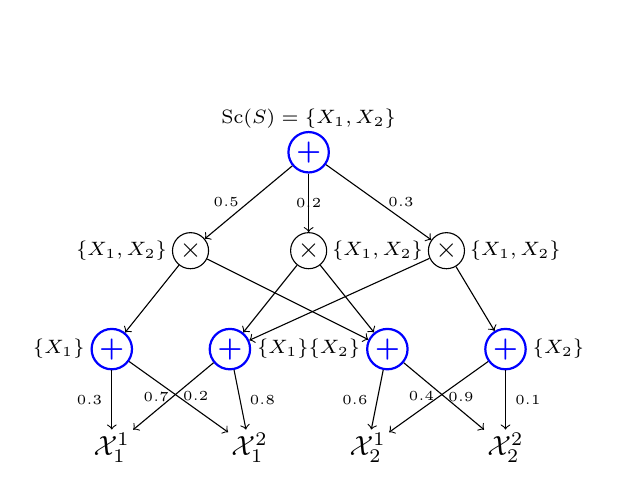
\begin{tikzpicture}
      \begin{scope}[every node/.style={circle,draw,inner sep=1pt}]
        \node[color=blue,thick,label={[label
          distance=-1.0cm]above:{\scriptsize$\Sc(S)=\{X_1,X_2\}$}}] (root) at (0, 0) {\textbf{+}};
        \node[label=left:{\scriptsize$\{X_1,X_2\}$}] (p1) at (-1.5, -1.25) {$\times$};
        \node[label=right:{\scriptsize$\{X_1,X_2\}$}] (p2) at (0, -1.25) {$\times$};
        \node[label=right:{\scriptsize$\{X_1,X_2\}$}] (p3) at (1.75, -1.25) {$\times$};
        \node[color=blue,thick,label=left:\scriptsize$\{X_1\}$] (s1) at (-2.5, -2.5) {\textbf{+}};
        \node[color=blue,thick,label=right:\scriptsize$\{X_1\}$] (s2) at (-1.0, -2.5) {\textbf{+}};
        \node[color=blue,thick,label=left:\scriptsize$\{X_2\}$] (s3) at (1.0, -2.5) {\textbf{+}};
        \node[color=blue,thick,label=right:\scriptsize$\{X_2\}$] (s4) at (2.5, -2.5) {\textbf{+}};
        \node[draw=none,fill=none,rectangle] (x11) at (-2.5, -3.75) {$\mathcal{X}_1^1$};
        \node[draw=none,fill=none,rectangle] (x12) at (-0.75, -3.75) {$\mathcal{X}_1^2$};
        \node[draw=none,fill=none,rectangle] (x21) at (0.75, -3.75) {$\mathcal{X}_2^1$};
        \node[draw=none,fill=none,rectangle] (x22) at (2.5, -3.75) {$\mathcal{X}_2^2$};
      \end{scope}

      \begin{scope}[every path/.style={->}]
        \draw (root) -- node[left]{\tiny$0.5$} (p1);
        \draw (root) -- node{\tiny$0.2$} (p2);
        \draw (root) -- node[right]{\tiny$0.3$} (p3);
        \draw (p1) -- (s1);
        \draw (p1) -- (s3);
        \draw (p2) -- (s2);
        \draw (p2) -- (s3);
        \draw (p3) -- (s2);
        \draw (p3) -- (s4);
        \draw (s1) -- node[left]{\tiny$0.3$} (x11);
        \draw (s1) -- node[left]{\tiny$0.7$} (x12);
        \draw (s2) -- node[right]{\tiny$0.2$} (x11);
        \draw (s2) -- node[right]{\tiny$0.8$} (x12);
        \draw (s3) -- node[left]{\tiny$0.6$} (x21);
        \draw (s3) -- node[left]{\tiny$0.4$} (x22);
        \draw (s4) -- node[right]{\tiny$0.9$} (x21);
        \draw (s4) -- node[right]{\tiny$0.1$} (x22);
      \end{scope}
    \end{tikzpicture}
  \end{center}
\end{frame}

\begin{frame}
  \frametitle{Consistency}
  \begin{definition}[Consistency]~\\
    An SPN $S$ is said to be consistent, iff no variable appears with a value $v$ in one child of a
    product node, and valued $u$, with $u\neq v$, in another.
  \end{definition}

  \begin{center}
    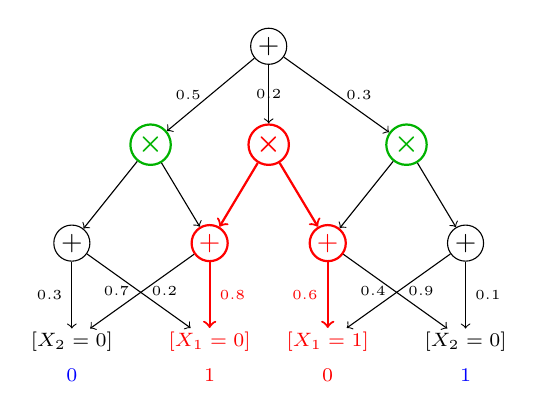
\begin{tikzpicture}
      \begin{scope}[every node/.style={circle,draw,inner sep=1pt}]
        \node (root) at (0, 0) {+};
        \node[color=black!30!green,thick] (p1) at (-1.5, -1.25) {$\boldsymbol{\times}$};
        \node[color=red,thick] (p2) at (0, -1.25) {$\boldsymbol{\times}$};
        \node[color=black!30!green,thick] (p3) at (1.75, -1.25) {$\boldsymbol{\times}$};
        \node (s1) at (-2.5, -2.5) {+};
        \node[color=red,thick] (s2) at (-0.75, -2.5) {+};
        \node[color=red,thick] (s3) at (0.75, -2.5) {+};
        \node (s4) at (2.5, -2.5) {+};
        \node[label={[label
          distance=0.1cm,color=blue]below:{\scriptsize$0$}},draw=none,fill=none,rectangle] (x11) at
          (-2.5, -3.75) {\scriptsize$[X_2=0]$};
        \node[color=red,thick,label={[label
          distance=0.1cm,color=red]below:{\scriptsize$1$}},draw=none,fill=none,rectangle] (x12) at
          (-0.75, -3.75) {\scriptsize$[X_1=0]$};
        \node[color=red,thick,label={[label
          distance=0.1cm,color=red]below:{\scriptsize$0$}},draw=none,fill=none,rectangle] (x21) at
          (0.75, -3.75) {\scriptsize$[X_1=1]$};
        \node[label={[label
          distance=0.1cm,color=blue]below:{\scriptsize$1$}},draw=none,fill=none,rectangle] (x22) at
          (2.5, -3.75) {\scriptsize$[X_2=0]$};
      \end{scope}

      \begin{scope}[every path/.style={->}]
        \draw (root) -- node[left]{\tiny$0.5$} (p1);
        \draw (root) -- node{\tiny$0.2$} (p2);
        \draw (root) -- node[right]{\tiny$0.3$} (p3);
        \draw (p1) -- (s1);
        \draw (p1) -- (s2);
        \draw[thick,color=red] (p2) -- (s2);
        \draw[thick,color=red] (p2) -- (s3);
        \draw (p3) -- (s3);
        \draw (p3) -- (s4);
        \draw (s1) -- node[left]{\tiny$0.3$} (x11);
        \draw (s1) -- node[left]{\tiny$0.7$} (x12);
        \draw (s2) -- node[right]{\tiny$0.2$} (x11);
        \draw[thick,color=red] (s2) -- node[right]{\tiny$0.8$} (x12);
        \draw[thick,color=red] (s3) -- node[left]{\tiny$0.6$} (x21);
        \draw (s3) -- node[left]{\tiny$0.4$} (x22);
        \draw (s4) -- node[right]{\tiny$0.9$} (x21);
        \draw (s4) -- node[right]{\tiny$0.1$} (x22);
      \end{scope}
    \end{tikzpicture}
  \end{center}\vspace{-1.0cm}

  \begin{equation*}
    X=\{X_1=0,X_2=1\}
  \end{equation*}

\end{frame}

\begin{frame}
  \frametitle{Decomposability}

  \begin{definition}[Decomposability]~\\
    An SPN is decomposable iff no variable appears in more than one child of a product node (i.e.
    scopes are disjoint).
  \end{definition}\vspace{-0.5cm}

  \begin{center}
    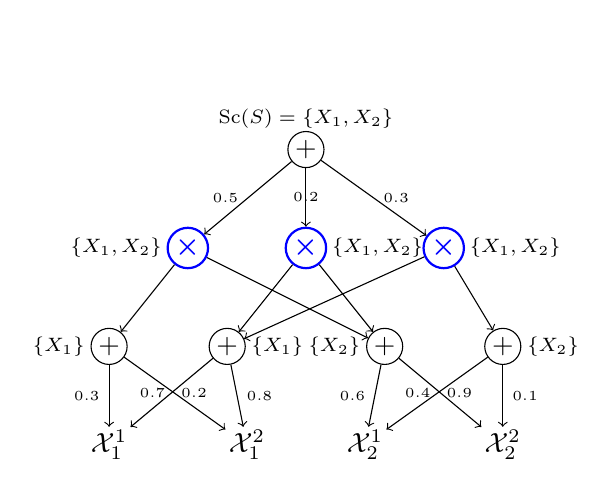
\begin{tikzpicture}
      \begin{scope}[every node/.style={circle,draw,inner sep=1pt}]
        \node[label={[label distance=-1.0cm]above:{\scriptsize$\Sc(S)=\{X_1,X_2\}$}}] (root) at (0, 0) {+};
        \node[color=blue,thick,label=left:{\scriptsize$\{X_1,X_2\}$}] (p1) at (-1.5, -1.25)
          {$\boldsymbol{\times}$};
        \node[color=blue,thick,label=right:{\scriptsize$\{X_1,X_2\}$}] (p2) at (0, -1.25)
          {$\boldsymbol{\times}$};
        \node[color=blue,thick,label=right:{\scriptsize$\{X_1,X_2\}$}] (p3) at (1.75, -1.25)
          {$\boldsymbol\times$};
        \node[label=left:\scriptsize$\{X_1\}$] (s1) at (-2.5, -2.5) {+};
        \node[label=right:\scriptsize$\{X_1\}$] (s2) at (-1.0, -2.5) {+};
        \node[label=left:\scriptsize$\{X_2\}$] (s3) at (1.0, -2.5) {+};
        \node[label=right:\scriptsize$\{X_2\}$] (s4) at (2.5, -2.5) {+};
        \node[draw=none,fill=none,rectangle] (x11) at (-2.5, -3.75) {$\mathcal{X}_1^1$};
        \node[draw=none,fill=none,rectangle] (x12) at (-0.75, -3.75) {$\mathcal{X}_1^2$};
        \node[draw=none,fill=none,rectangle] (x21) at (0.75, -3.75) {$\mathcal{X}_2^1$};
        \node[draw=none,fill=none,rectangle] (x22) at (2.5, -3.75) {$\mathcal{X}_2^2$};
      \end{scope}

      \begin{scope}[every path/.style={->}]
        \draw (root) -- node[left]{\tiny$0.5$} (p1);
        \draw (root) -- node{\tiny$0.2$} (p2);
        \draw (root) -- node[right]{\tiny$0.3$} (p3);
        \draw (p1) -- (s1);
        \draw (p1) -- (s3);
        \draw (p2) -- (s2);
        \draw (p2) -- (s3);
        \draw (p3) -- (s2);
        \draw (p3) -- (s4);
        \draw (s1) -- node[left]{\tiny$0.3$} (x11);
        \draw (s1) -- node[left]{\tiny$0.7$} (x12);
        \draw (s2) -- node[right]{\tiny$0.2$} (x11);
        \draw (s2) -- node[right]{\tiny$0.8$} (x12);
        \draw (s3) -- node[left]{\tiny$0.6$} (x21);
        \draw (s3) -- node[left]{\tiny$0.4$} (x22);
        \draw (s4) -- node[right]{\tiny$0.9$} (x21);
        \draw (s4) -- node[right]{\tiny$0.1$} (x22);
      \end{scope}
    \end{tikzpicture}
  \end{center}
\end{frame}

\begin{frame}
  \frametitle{Decomposability vs Consistency}

  \textbf{Decomposability} implies \textbf{consistency}.
  \vfill

  But \textbf{decomposability} is much easier for learning, and allows for an interpretation of
  product nodes as \emph{independencies} between variables.
  \vfill

  \cite{theoretical-spn} shows \textbf{decomposable} SPNs are as representable as solely
  \textbf{consistent} ones.
\end{frame}

\begin{frame}
  \frametitle{Probability of evidence}

  Single backward pass computes $S(X=\{X_1=0\})=0.31$. Linear on the number of edges.

  \begin{figure}
    \centering\includegraphics[height=0.6\textheight]{imgs/sample_spn_prob.png}
  \end{figure}

  Marginalizing variables means taking the mode of the corresponding distributions.
\end{frame}

\begin{frame}
  \frametitle{Maximum a posteriori probability}

  Replace sums with max nodes. Backward pass followed by forward pass computes \textbf{approximate}
  most probable explanation, i.e. find $M(E)=\argmax_{x\in X} P(X=x, E)$.

  \begin{figure}
    \centering\includegraphics[height=0.6\textheight]{imgs/sample_mpn_prob.png}
  \end{figure}
\end{frame}

\begin{frame}
  \frametitle{Learning}

  \textbf{Structure}
  \begin{itemize}
    \item PD-Dense architecture (\cite{poon-domingos})
    \item \textbf{Clustering on Variables} (\cite{clustering})
    \item \textbf{Gens-Domingos LearnSPN} (\cite{gens-domingos})
    \item Using deep learning techniques (\cite{deep-learn-spn})
    \item many others\ldots
  \end{itemize}

  \textbf{Weights}
  \begin{itemize}
    \item \textbf{Generative and discriminative gradient descent}
    \item Generative Expectation-Maximization
    \item Extended Baum-Welch (\cite{baum-welch})
    \item many others\ldots
  \end{itemize}
\end{frame}

\begin{frame}
  \frametitle{Dennis-Ventura architecture}

  \textbf{Idea:}\\
  \begin{itemize}
    \item Sums are latent variables;
    \item Products are statistical independencies;
    \item A set of sums describes a \emph{region}, and each sum is a potential semantical
      interpretation of its scope within a region;
    \item A set of products is a \emph{partitioning} of regions.
  \end{itemize}

  \textbf{In practice:}\\
  \begin{itemize}
    \item Regions are clusters of similar pixels;
    \item Products partition regions into subregions;
    \item Use $k$-clustering for both tasks.
  \end{itemize}
\end{frame}

\begin{frame}
  \frametitle{Dennis-Ventura architecture}

  \begin{figure}[h]
    \centering\includegraphics{imgs/trans_dv.png}
    \captionsetup{justification=centering}
    \caption*{\cite{clustering}}
  \end{figure}

  \begin{itemize}
    \item $2$-clustering on \textbf{instances} to create regions.
    \item $2$-clustering on \textbf{variables} to partition regions into two subregions.
  \end{itemize}
\end{frame}

\begin{frame}
  \frametitle{Dennis-Ventura architecture for classification}

  Let $k$ be the number of classification labels (in our case $k=3$).

  \begin{description}
    \item[Original algorithm:]~\\
      \begin{itemize}
        \item Initial $k$-clustering to determine sub-SPNs for each label;
        \item Each sub-SPN should ideally model a single label;
        \item Does not scale when number of variables is high;
        \item Clustering might not guarantee sub-SPNs are split by classification labels.
      \end{itemize}
    \item[Our version:]~\\
      \begin{itemize}
        \item Explicitly create sub-SPNs for each label;
        \item Each sub-SPN is trained with only data with assigned label;
      \end{itemize}
  \end{description}
\end{frame}

\begin{frame}
  \frametitle{Dennis-Ventura architecture for classification}

  Each product child of root acts as a switch. When the classification variable $Y=y$, all other
  sub-SPNs $S|Y=u$, $u\neq y$ are ``switched off'' and have value zero.

  \begin{figure}[h]
    \centering\includegraphics[width=0.9\textwidth]{imgs/classarch.png}
  \end{figure}

  \centering\textbf{Result:} much better performance compared to original.
\end{frame}

\begin{frame}
  \frametitle{Gens-Domingos architecture}

  \textbf{Idea:}\\
  \begin{itemize}
    \item Sums cluster similar instances/images;
    \item Products are independencies between variables;
    \item Recursively split dataset by instances or variables;
    \item Base case is a univariate distribution.
  \end{itemize}

  \textbf{In practice:}\\
  \begin{itemize}
    \item Clustering algorithm for sums ($k$-means, DBSCAN, ...);
    \item Statistical independence test for products ($\chi^2$, $G$-test, ...);
    \item Multinomial or mixture of gaussians for leaves.
  \end{itemize}
\end{frame}

\begin{frame}
  \frametitle{LearnSPN}

  \begin{algorithm}[H]
    \caption{\code{LearnSPN}: Gens-Domingos structure learning schema}
    \begin{algorithmic}[1]
      \Require Set of instances $D$ and scope $X$
      \Ensure SPN structure learned from $D$ and $X$
      \If{$|X|=1$}
        \State \textbf{return} univariate distribution over $D_X$
      \EndIf%
      \State Partition $X$ into $P_1,P_2,\ldots,P_m$ st $\forall i, j$, $i\neq j$, $P_i\indep P_j$
      \If{$m>1$}
        \State \textbf{return} $\prod_i$\mcode{LearnSPN$(D,P_i)$}
      \EndIf%
      \State Cluster $D$ such that $Q_1,Q_2,\ldots,Q_n$ are $D$'s clusters
      \State \textbf{return} $\sum_i\frac{|Q_i|}{|D|}$\mcode{LearnSPN$(Q_i,X)$}
    \end{algorithmic}
  \end{algorithm}
\end{frame}

\begin{frame}
  \frametitle{Visualizing the Gens-Domingos architecture}

  \begin{figure}[h]
    \centering\includegraphics[width=0.9\textwidth]{imgs/learnspn.png}
    \captionsetup{justification=centering}
    \caption*{\cite{gens-domingos}}
  \end{figure}
\end{frame}

\begin{frame}
  \frametitle{Parameter learning}

  \scriptsize
  \begin{table}[h]
    \centering
    \begin{tabular}{l|l}
      \hline
      \multicolumn{1}{c}{\bfseries Inference} & \multicolumn{1}{c}{\bfseries Weight updates}\\
      \hline & \\
      \textbf{Soft} & \(\displaystyle \Delta w_{n,j}=\eta\ddspn{S}{w_{n,j}}(X, Y)-2\lambda w_{n,j} \) \\
      & \\
      \textbf{Hard} & \(\displaystyle \Delta w_{n,j}=\eta\frac{c_{n,j}}{w_{n,j}}-2\lambda w_{n,j} \) \\
      & \\
      \hline
    \end{tabular}
    \captionsetup{justification=centering}
    \caption*{\scriptsize Generative gradient descent weight updates with L2 regularization.}
  \end{table}
  \begin{table}[h]
    \centering
    \begin{tabular}{l|l}
      \hline
      \multicolumn{1}{c}{\bfseries Inference} & \multicolumn{1}{c}{\bfseries Weight updates}\\
      \hline & \\
      \textbf{Soft} & \(\displaystyle \Delta
        w_{n,j}=\eta\left(\frac{1}{S(Y,X)}\ddspn{S(Y,X)}{w_{n,j}}-\frac{1}{S(X)}
          \ddspn{S(X)}{w_{n,j}}\right)-2\lambda w_{n,j} \) \\
      & \\
      \textbf{Hard} & \(\displaystyle \Delta w_{n,j}=\eta\frac{\Delta c_{n,j}}{w_{n,j}}-2\lambda w_{n,j} \) \\
      & \\
      \hline
    \end{tabular}
    \captionsetup{justification=centering}
    \caption*{\scriptsize Discriminative gradient descent weight updates with L2 regularization.}
  \end{table}
\end{frame}

\begin{frame}
  \frametitle{Gradient diffusion}

  {
    \footnotesize
    \textbf{Soft gradient:} the deeper the network, the faster the signal dwindles to zero.\\
    \textbf{Hard gradient:} derivatives are actually counts, so signal stays constant.
  }

  \begin{figure}[h]
    \centering
    \begin{subfigure}[b]{0.45\linewidth}
      \centering\includegraphics[width=\textwidth]{imgs/softgrad.png}
      \captionsetup{justification=centering}
      \caption{Soft gradient}
    \end{subfigure}
    \begin{subfigure}[b]{0.45\linewidth}
      \centering\includegraphics[width=\textwidth]{imgs/hardgrad.png}
      \captionsetup{justification=centering}
      \caption{Hard gradient}
    \end{subfigure}
  \end{figure}
\end{frame}

\begin{frame}
  \frametitle{Hard discriminative gradient}

  We want to optimize $P(Y|X)$, as ours is a classification task. Using hard gradient helps with
  the gradient diffusion problem.

  \begin{figure}[h]
    \centering
    \begin{minipage}{0.3\textwidth}
      \includegraphics[width=\linewidth]{imgs/hard_diff_0.png}
      \captionsetup{justification=centering}
      \caption*{$\ddspn{}{W}\log M(Y,X)$}
    \end{minipage}
    $-$
    \begin{minipage}{0.3\textwidth}
      \includegraphics[width=\linewidth]{imgs/hard_diff_1.png}
      \captionsetup{justification=centering}
      \caption*{$\ddspn{}{W}\log M(X)$}
    \end{minipage}
    $=$
    \begin{minipage}{0.3\textwidth}
      \includegraphics[width=\linewidth]{imgs/hard_diff_2.png}
      \captionsetup{justification=centering}
      \caption*{$\nabla\log\tilde{P}(Y|X)$}
    \end{minipage}
  \end{figure}
\end{frame}

\section{Self-Driving}

\begin{frame}
  \frametitle{The task}

  Given a track, bot must be able to autonomously complete the whole course without going off road.

  \begin{figure}[h]
    \centering\includegraphics[width=0.8\textwidth]{imgs/track_1.png}
  \end{figure}

  Inspired by~\cite{self-driving}, which was itself inspired by~\cite{nvidia-driving}.
\end{frame}

\begin{frame}
  \frametitle{Dataset}

  Dataset used: \cite{self-driving}

  \begin{figure}
    \centering\includegraphics[height=0.5\textheight]{imgs/montage_raw.png}
  \end{figure}

  Lane tracking dataset with $80\times 45$ RGB images. Each labeled with either UP, LEFT or RIGHT.
\end{frame}

\begin{frame}
  \frametitle{Self-driving as image classification}

  Let $X=\{X_0,X_1,\ldots,X_{n-1}\}$ be an \textbf{image}. Every $X_i=x_i$ refers to the $i$-th
  pixel with a grayscale intensity of $x_i$.

  Let $Y=\{\Up,\Left,\Right\}$ be the \textbf{classification variable}.

  \begin{figure}
    \begin{subfigure}{0.3\linewidth}
      \centering\includegraphics{imgs/sample_left.png}
      \captionsetup{justification=centering}
      \caption*{LEFT}
    \end{subfigure}
    \begin{subfigure}{0.3\linewidth}
      \centering\includegraphics{imgs/sample_up.png}
      \captionsetup{justification=centering}
      \caption*{UP}
    \end{subfigure}
    \begin{subfigure}{0.3\linewidth}
      \centering\includegraphics{imgs/sample_right.png}
      \captionsetup{justification=centering}
      \caption*{RIGHT}
    \end{subfigure}
  \end{figure}

  The entire scope of variables is $X\cup \{Y\}$.

  \vfill\centering\textbf{Objective:} $\argmax_{y\in Y} P(Y=y|X)$
\end{frame}

\begin{frame}
  \frametitle{Pre-processing}

  \textbf{Pipeline:}

  \centering{original RGB image $\to$ grayscale $\to$ some $T$ transformation.}

  \flushleft Three transformations tested:
  \begin{enumerate}
    \item Otsu binarization (\cite{otsu})
    \item Quantization (resolution downscaling)
    \item Histogram equalization
  \end{enumerate}

  \begin{figure}
    \begin{subfigure}{0.3\linewidth}
      \centering\includegraphics{imgs/binary_up.png}
      \captionsetup{justification=centering}
      \caption*{1}
    \end{subfigure}
    \begin{subfigure}{0.3\linewidth}
      \centering\includegraphics{imgs/trans_up.png}
      \captionsetup{justification=centering}
      \caption*{2}
    \end{subfigure}
    \begin{subfigure}{0.3\linewidth}
      \centering\includegraphics{imgs/eq_up.png}
      \captionsetup{justification=centering}
      \caption*{3}
    \end{subfigure}
  \end{figure}
\end{frame}

\begin{frame}
  \frametitle{The problems with binarization}

  Hard threshold binarization produces lots of noise!

  \begin{figure}
    \begin{subfigure}{0.3\linewidth}
      \centering\includegraphics{imgs/binary_left_h.png}
      \captionsetup{justification=centering}
    \end{subfigure}
    \begin{subfigure}{0.3\linewidth}
      \centering\includegraphics{imgs/binary_up_h.png}
      \captionsetup{justification=centering}
    \end{subfigure}
    \begin{subfigure}{0.3\linewidth}
      \centering\includegraphics{imgs/binary_right_h.png}
      \captionsetup{justification=centering}
    \end{subfigure}
  \end{figure}

  \begin{figure}
    \begin{subfigure}{0.3\linewidth}
      \centering\includegraphics{imgs/binary_left.png}
      \captionsetup{justification=centering}
      \caption*{LEFT}
    \end{subfigure}
    \begin{subfigure}{0.3\linewidth}
      \centering\includegraphics{imgs/binary_up.png}
      \captionsetup{justification=centering}
      \caption*{UP}
    \end{subfigure}
    \begin{subfigure}{0.3\linewidth}
      \centering\includegraphics{imgs/binary_right.png}
      \captionsetup{justification=centering}
      \caption*{RIGHT}
    \end{subfigure}
  \end{figure}

  Otsu's works well, but takes too long!
\end{frame}

\begin{frame}
  \frametitle{Berry}

  \textbf{Raspberry Pi 3 Model B --- Berry}
  \begin{description}
    \item[CPU:] Quad Core 1.2GHz Broadcom BCM2837 64bit ARMv7
    \item[Memory:] 1GB RAM
    \item[Storage:] 16GB SSD
  \end{description}

  \begin{figure}
    \centering\includegraphics[height=0.4\textheight]{imgs/berry.png}
  \end{figure}
\end{frame}

\begin{frame}
  \frametitle{Brick}

  \textbf{Lego Mindstorms NXT v2 --- Brick}
  \begin{description}
    \item[CPU:] Atmel AT91SAM7S256 48MHz 32bit ARMv4
    \item[Memory:] 64KB RAM
    \item[Storage:] 256KB Flash
  \end{description}

  \begin{figure}
    \centering\includegraphics[height=0.4\textheight]{imgs/brick.png}
  \end{figure}
\end{frame}

\begin{frame}
  \frametitle{Robot}

  \textbf{Berry} handles inference, passing predicted label to \textbf{Brick}.

  \textbf{Brick} handles motors according to label received from \textbf{Berry}.

  \begin{figure}
    \centering\includegraphics[height=0.5\textheight]{imgs/robot.png}
  \end{figure}

  \centering Message passing through USB cable.
\end{frame}

\begin{frame}
  \frametitle{Evaluation approaches}

  \begin{description}
    \item[\cite{self-driving}:]~\\
      \begin{itemize}
        \item Asynchronous;
        \item Actions are computed and passed to bot;
        \item Only moves when action is available, idles otherwise;
        \item Bot moves a \emph{fixed} distance;
        \item \emph{Accuracy} ``matters more'' than \emph{inference speed}.
      \end{itemize}
    \item[Our approach (real-time):]~\\
      \begin{itemize}
        \item Bot is always moving;
        \item Actions are computed in real-time;
        \item Action runs indefinitely until told otherwise;
        \item Bot movement depends on \emph{prediction speed};
        \item Balance between \emph{accuracy} and \emph{inference speed};
        \item More ``realistic''.
      \end{itemize}
  \end{description}
\end{frame}

\section{Driving with SPNs}

\begin{frame}
  \frametitle{Modelling}

  Every pixel $X_i$ is a variable in the distribution represented by the SPN, i.e. no additional
  feature extraction, end-to-end.

  Two architectures:
  \begin{description}
    \item[GD:] LearnSPN with $k$-means and $G$-test
    \item[DV:] Clustering on Variables
  \end{description}
  Three weight setups:
  \begin{description}
    \item[g:] Generative gradient descent
    \item[d:] Discriminative gradient descent
    \item[s:] Proportional weights for GD, random weights for DV
  \end{description}
\end{frame}

\begin{frame}
  \frametitle{Accuracy}
  \footnotesize
  \begin{table}[h]
    \centering
    \begin{tabular}{l|c|c|c|c|c|c}
      \hline
      \multicolumn{1}{c}{\bfseries Accuracy (\%)} & \multicolumn{1}{c}{\bfseries DV+g} &
      \multicolumn{1}{c}{\bfseries DV+d} & \multicolumn{1}{c}{\bfseries DV+s} &
      \multicolumn{1}{c}{\bfseries GD+g} & \multicolumn{1}{c}{\bfseries GD+d} &
      \multicolumn{1}{c}{\bfseries GD+s}\\
      \hline
      $B$         & 78.8 & 78.8 & 78.8 & 82.8 & 83.8 & 85.0\\
      $Q_2$       & 78.6 & 78.0 & 78.0 & 78.6 & 80.4 & 79.4\\
      $Q_2+E$     & 76.6 & 76.6 & 76.8 & 79.6 & 82.8 & 81.8\\
      $Q_3$       & 77.4 & 77.4 & 77.4 & 77.6 & 80.2 & 79.8\\
      $Q_3+E$     & 70.4 & 76.6 & 76.6 & 79.2 & 81.2 & 77.4\\
      $Q_4$       & 78.2 & 78.4 & 78.2 & 76.0 & \textbf{78.2} & 76.4\\
      $Q_4+E$     & 76.6 & 76.6 & 76.8 & 76.0 & 74.6 & 80.6\\
      $Q_5$       & 77.8 & 78.4 & 78.4 & 77.6 & 74.0 & 73.8\\
      $Q_5+E$     & 76.6 & 76.6 & 76.6 & 72.0 & 72.8 & 72.0\\
      $Q_6$       & 77.4 & 78.4 & 78.4 & 75.2 & \textbf{74.4} & 72.0\\
      $Q_6+E$     & 76.0 & 76.4 & 76.4 & 73.0 & 75.0 & 73.6\\
      $Q_7$       & 78.2 & 78.4 & 78.4 & 62.8 & 72.2 & 71.4\\
      $Q_7+E$     & 76.2 & 76.4 & 76.4 & 70.6 & 71.4 & 71.6\\
      $\emptyset$ & 78.0 & 78.4 & 78.4 & 62.4 & \textbf{62.4} & 62.4\\
      $E$         & 76.4 & 76.4 & 76.4 & 60.4 & 60.0 & 61.2\\
    \end{tabular}
  \end{table}
\end{frame}

\begin{frame}
  \frametitle{Inference time}
  \footnotesize
  \begin{table}[h]
    \centering
    \begin{tabular}{l|c|c|c|c|c|c}
      \hline
      \multicolumn{1}{c}{\bfseries Inference (secs)} & \multicolumn{1}{c}{\bfseries DV+g} &
      \multicolumn{1}{c}{\bfseries DV+d} & \multicolumn{1}{c}{\bfseries DV+s} &
      \multicolumn{1}{c}{\bfseries GD+g} & \multicolumn{1}{c}{\bfseries GD+d} &
      \multicolumn{1}{c}{\bfseries GD+s}\\
      \hline
      $B$         & 0.23 & 0.25 & 0.25 & 0.38 & 0.37 & 0.31 \\
      $Q_2$       & 0.22 & 0.24 & 0.23 & 0.28 & 0.34 & 0.16 \\
      $Q_2+E$     & 0.22 & 0.23 & 0.23 & 0.38 & 0.30 & 0.27 \\
      $Q_3$       & 0.22 & 0.23 & 0.22 & 0.22 & 0.32 & 0.17 \\
      $Q_3+E$     & 0.22 & 0.23 & 0.22 & 0.34 & 0.32 & 0.31 \\
      $Q_4$       & 0.22 & 0.22 & 0.23 & 0.16 & \textbf{0.17} & 0.13 \\
      $Q_4+E$     & 0.23 & 0.27 & 0.29 & 0.13 & 0.14 & 0.13 \\
      $Q_5$       & 0.22 & 0.26 & 0.28 & 0.07 & 0.05 & 0.02 \\
      $Q_5+E$     & 0.22 & 0.29 & 0.25 & 0.05 & 0.05 & 0.02 \\
      $Q_6$       & 0.23 & 0.24 & 0.23 & 0.04 & \textbf{0.05} & 0.01 \\
      $Q_6+E$     & 0.22 & 0.24 & 0.28 & 0.03 & 0.04 & 0.02 \\
      $Q_7$       & 0.23 & 0.23 & 0.26 & 0.03 & 0.01 & 0.01 \\
      $Q_7+E$     & 0.22 & 0.26 & 0.24 & 0.01 & 0.01 & 0.01 \\
      $\emptyset$ & 0.22 & 0.26 & 0.23 & 0.02 & \textbf{0.01} & 0.01 \\
      $E$         & 0.23 & 0.23 & 0.22 & 0.01 & 0.01 & 0.02 \\
    \end{tabular}
  \end{table}
\end{frame}

\begin{frame}
  \frametitle{Chosen models}

  \begin{description}
    \item[Model 1:] $Q_4$, \textbf{GD+d}
      \begin{description}
        \item[Accuracy:] 78.2\%
        \item[Desktop time:] 170ms
        \item[Berry time:] 700ms
      \end{description}
    \item[Model 2:] $Q_6$, \textbf{GD+d}
      \begin{description}
        \item[Accuracy:] 74.4\%
        \item[Desktop time:] 50ms
        \item[Berry time:] 150ms
      \end{description}
    \item[Model 3:] $\emptyset$, \textbf{GD+d}
      \begin{description}
        \item[Accuracy:] 62.4\%
        \item[Desktop time:] $<$ 10ms
        \item[Berry time:] 75ms
      \end{description}
  \end{description}
\end{frame}

\begin{frame}
  \frametitle{The accuracy vs speed dilemma}

  Fundamental to find a balance between \textbf{accuracy} and \textbf{speed}.

  \large
  \begin{align*}
    &\hspace{-0.30cm}\textcolor{blue}{\boldsymbol\uparrow}\text{ Network complexity }&\implies\text{ }
    \textcolor{blue}{\boldsymbol\uparrow}\text{ Accuracy }&\implies\text{ }
    \textcolor{red}{\boldsymbol\downarrow}\text{ Inference speed}\\
    &\hspace{-0.30cm}\textcolor{blue}{\boldsymbol\uparrow}\text{ Inference speed }&\implies\text{ }
    \textcolor{red}{\boldsymbol\downarrow}\text{ Accuracy }&\implies\text{ }
    \textcolor{red}{\boldsymbol\downarrow}\text{ Network complexity}\\
  \end{align*}

  \normalsize

  How much accuracy can we sacrifice for speed, and still have a reliable and safe model?
\end{frame}

\begin{frame}
  \frametitle{Some interesting data}

  \begin{itemize}
    \item We used only 500 samples for training out of the total of 56172 images \textbf{(0.9\% of
      the dataset)}.
    \item With 1000 samples we had much more accurate models, but inference takes much longer.
    \item Gens-Domingos LearnSPN with DBSCAN for clustering:\\
      \begin{itemize}
        \item Only 500 training samples.
        \item Network 32 times bigger than $k$-means variant.
        \item Achieved \textbf{100\% accuracy} on all tests!
        \item Whopping \textbf{19.72 seconds} for inference on training computer.
      \end{itemize}
  \end{itemize}

\end{frame}

\begin{frame}
  \frametitle{Training}

  Training was done on an Intel i7-4500U CPU \@ 1.80 Hz.

  \begin{figure}[h]
    \centering
    \resizebox{\columnwidth}{!}{
      \begin{tikzpicture}
        \node[inner sep=0pt, label=Raw] (raw) at (0, 0)
          {\includegraphics{imgs/pipe_raw.png}};
        \node[inner sep = 0pt, right = 2.0cm of raw, label=Gray] (gray)
          {\includegraphics{imgs/pipe_gray.png}};
        \node[inner sep = 0pt, right = 2.0cm of gray, label=Binarized] (bin)
          {\includegraphics{imgs/pipe_bin.png}};
        \node[rectangle, rounded corners, draw, below = 2.0cm of gray,
          minimum size=2cm] (weights) {LearnWeight};
        \node[rectangle, rounded corners, draw, right = 2.0cm of weights,
          minimum size=2cm] (struct) {LearnStructure};
        \node[cylinder, shape border rotate=90, draw, left = 2.0cm of weights,
          label=below:SaveDisk, minimum width=2cm, minimum height=1cm] (save) {};
        \node[inner sep = 0.75cm, rectangle, dashed, draw, thick, fit=(raw) (gray) (bin),
          label=above:\textbf{Pre-processing}] (pp) {};
        \node[inner sep = 0.5cm, rectangle, dotted, draw, thick, fit=(struct) (weights) (save),
          label=above:\textbf{Training}] (train) {};
        \draw[->,thick] (raw.east) -- (gray.west);
        \draw[->,thick] (gray.east) -- (bin.west);
        \draw[->,thick] let \p1 = (train.east), \p2 = (pp.east) in
          (\p2) -- ($ (\p2) + (0.5, 0) $) -- ($ (\x2, \y1) + (0.5, 0) $) -- (\p1);
        \draw[->,thick] (struct.west) -- (weights.east);
        \draw[->,thick] (weights.west) -- (save.east);
      \end{tikzpicture}
    }
  \end{figure}

  Saved SPN was then passed to the Raspberry.
\end{frame}

\begin{frame}
  \frametitle{Inference pipeline}

  Rasberry has to:

  \begin{enumerate}
    \item Capture raw camera data;
    \item Convert data to grayscale;
    \item Apply transformation to image;
    \item Convert image into set of variable valuations, feeding SPN;
    \item Compute probabilities for each label (LEFT, RIGHT, UP);
    \item Send most probable label to Brick;
    \item Record camera feed with probabilities overlay.
  \end{enumerate}

  in \textbf{less than a second}!
\end{frame}

\begin{frame}
  \frametitle{Inference}

  Two possible options for computing $\argmax_y P(Y=y|X)$:
  \vfill

  \begin{enumerate}
    \item Approximately:\\
      \begin{itemize}
        \item Use MAP to compute most probable label in linear time.
        \item This could be an option when the SPN is big.
      \end{itemize}
    \item Exactly:\\
      \begin{itemize}
        \item Compute each $P(Y=y|X)$, $\forall y\in\Val(Y)$, get the max.
        \item Since $|\Val(Y)|$ is small, feasible.
      \end{itemize}
  \end{enumerate}
  \vfill

  We chose to compute the exact probabilities.
\end{frame}

\begin{frame}
  \frametitle{Optimizations}

  The Raspberry has four cores. Let's make use of them!

  \begin{description}[width=1cm]
    \item[CPU1:] Capture and process image data.
    \item[CPU2:] Compute probability of label LEFT.
    \item[CPU3:] Compute probability of label RIGHT.
    \item[CPU4:] Compute probability of label UP.
  \end{description}

  Surprisingly, \textbf{CPU1} often takes the longest.

\end{frame}

\begin{frame}
  \frametitle{Prediction}

  \begin{figure}[h]
    \centering
    \resizebox{\columnwidth}{!}{
      \begin{tikzpicture}
        \node[inner sep=0pt, label=Raw] (raw) at (0, 0)
          {\includegraphics{imgs/pipe_out_raw.png}};
        \node[inner sep = 0pt, right = 2.0cm of raw, label=Gray] (gray)
          {\includegraphics{imgs/pipe_out_gray.png}};
        \node[inner sep = 0pt, right = 2.0cm of gray, label=Binarized] (bin)
          {\includegraphics{imgs/pipe_out_bin.png}};
        \node[inner sep = 0.75cm, rectangle, dashed, draw, thick, fit=(raw) (gray) (bin),
          label=above:\textbf{Pre-processing}] (pp) {};
        \node[cylinder, shape border rotate=90, draw, below = 2.0cm of raw,
          label=below:LoadDisk, minimum width=2cm, minimum height = 1cm] (load) {};
        \node[rectangle, rounded corners, draw, right = 2.0cm of load,
          minimum size=2cm] (build) {BuildSPN};
        \node[rectangle, rounded corners, draw, right = 2.0cm of build, right = 3.0cm of build,
          minimum size=2cm] (infer) {Inference};
        \node[inner sep = 0.5cm, rectangle, dotted, draw, thick, fit=(load) (build),
          label=below:\textbf{SPN loading}] (create) {};
        \node[below = 1.0cm of infer] (pred) {Predicted: RIGHT};
        \draw[->,thick] (raw.east) -- (gray.west);
        \draw[->,thick] (gray.east) -- (bin.west);
        \draw[->,thick] let \p1 = (infer.east), \p2 = (pp.east) in
          (\p2) -- ($ (\p2) + (0.5, 0) $) -- ($ (\x2, \y1) + (0.5, 0) $) -- (\p1);
        \draw[->,thick] (load) -- (build);
        \draw[->,thick] (create) -- (infer);
        \draw[->,thick] (infer) -- (pred);
      \end{tikzpicture}
    }
  \end{figure}
\end{frame}

\begin{frame}
  \frametitle{Comparison to neural networks}

  Comparison to~\cite{self-driving}:

  \begin{table}
    \centering
    \begin{tabular}{l|c|c}
      \textbf{Model} & \textbf{Accuracy (\%)} & \textbf{Speed (seconds)}\\
      \hline
      DFN & 81.3 & $\approx$1.35\\
      CNN & 80.6 & $\approx$1.35\\
      $Q_4$, GD-SPN+d & 78.2 & $\approx$0.70\\
      $Q_6$, GD-SPN+d & 74.4 & $\approx$0.15\\
      GD-SPN+d & 62.4 & $\approx$0.07
    \end{tabular}
  \end{table}

  Neural networks were more accurate, but real-time prediction with them is unfeasible.\\~\\

  Our implementation did not make use of the GPU, which could increase speed dramatically.

\end{frame}

\begin{frame}
  \frametitle{``Real world'' scenario}

  \footnotesize\centering\textbf{\href{https://youtu.be/vhpWQDX2cQU}{Mobile Robot Self-Driving Through Image Classification Using
  Discriminative Learning of Sum-Product Networks --- YouTube}}
  (\url{https://youtu.be/vhpWQDX2cQU})
\end{frame}

\begin{frame}
  \frametitle{Implementation}
  \centering
  \large\textbf{Inference and learning:} \href{https://github.com/RenatoGeh/gospn}{GoSPN}
  (\url{https://github.com/RenatoGeh/gospn})\\~\\

  \textbf{Mobile robot implementation:} \href{https://github.com/RenatoGeh/godrive}{GoDrive}
  (\url{https://github.com/RenatoGeh/godrive})

\end{frame}

\begin{frame}
  \frametitle{Full thesis}

  \centering\large
  \textbf{Full thesis}:\\\url{https://www.ime.usp.br/~renatolg/mac0499}

\end{frame}

\begin{frame}[standout]
  \textbf{Thank you.\\~\\Questions?}
\end{frame}

\begin{frame}[t,allowframebreaks]
  \frametitle{References}
  \printbibliography[heading=none]
\end{frame}

\end{document}
